\documentclass[11pt]{article}
\usepackage{amsmath, amssymb, amsthm, graphicx, enumerate, listings}
\usepackage[margin=1in]{geometry}
\usepackage{hyperref}

\lstset{
	    language=bash,
		        keywordstyle=\ttfamily
}

\title{Parallelzing an All-Pairs Shortest Path Algorithm}

\author{Bangrui Chen (bc496), Markus Salasoo (ms933), and Calvin Wylie (cjw278)}

\begin{document}

\maketitle

\section*{Introduction}

In this report we describe the implementation and tuning of a parallel all-pairs shortest
path algorithm.

\section*{Profiling the given code}

\subsection*{VTune Amplifier}
Given a working implementation of parallelized Floyd-Warshall algorithm, we can further increase the performance by profiling the computation. This will identify areas in the code that run much slower than the rest, giving opportunities to implement speedups. We used the VTune Amplifier to profile our code, calling our executable through the profiler with
\begin{lstlisting}[language=bash]
amplxe-cl -collect hotspots ./path.x
\end{lstlisting}
\begin{figure}[ht!]
\centering
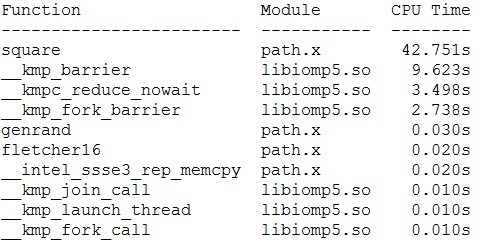
\includegraphics{vtuneResults.jpg}
\end{figure}
The hotspots analysis results tell us that the most expensive compute-time occurs in $square()$. This is expected because $square()$ is the only method with nested loops carrying out the algorithm ($write\_matrix()$ only prints values before and after our algorithm has run).\newline\newline
There are two other methods in our top CPU time list from path.c however any effort put towards optimizing those would not be well spent because they are orders of magnitude faster than $square()$.\newline\newline
We can dig deeper into $square()$'s performance by running the command
\begin{lstlisting}[language=bash]
amplxe-cl -report hotspots -source-object function="square"
\end{lstlisting}
\begin{figure}[ht!]
\centering
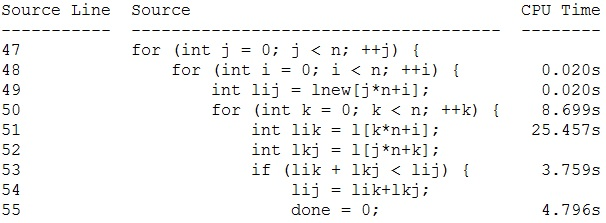
\includegraphics{squareProfiled.jpg}
\end{figure}
This tells us the CPU time spent at many points within the method. We can see the majority of the time is spent retrieving a value from the array in the innermost loop. Observe that the matrix accesses are not optimized because we fetch non-contiguous memory each iteration and it is taking a long time. We can re-order the loops to better access our desired values and improve the runtime.\newline\newline

\subsection*{Vectorization Report}
If we analyze the given code's vectorization report, we can try to adjust some code to take advantage of the compiler's vectorization capabilites. Compiling the code with flags
\begin{lstlisting}[language=bash]
-qopt-report=5 -qopt-report-phase=vec
\end{lstlisting}
will produce a report summarizing the compiler's ability to vectorize our code. In summary, the given code path.c is reported to be mostly vectorized. Most estimated potential speedup values were greater than 5, yielding a large factor of speedup. Some loops were not vectorizeable because they contained print statements. Another non-vectorizeable loop was in $fletcher16()$, but our profiling results show this method to be insignificant in runtime comparison to $square()$ so we will focus our efforts towards $square()$.


\section*{OpenMP Scaling Study}
We did both strong scaling and weak scaling study using the provided OpenMP code.

\subsection*{Strong Scaling}
In the strong scaling, we compare parallel to serial time for a fixed size problem. Since the graph is randomly generated, for each experiment, we did 10 simulation and use the average time as their running time. Here we choose the problem size $n=2000$ and the speedup is summarized in left plot of Figure~\ref{scaling}. As can be seen from the left plot of Figure~\ref{scaling}, when we increase the number of threads from 1 to 12, the speed up grows linearly with respect to the number of threads. After 12 threads, the speedup doesn't grow linearly due to the excess amount of overheading and synchronization.

\begin{figure}
\caption{scaling study}
\label{scaling}
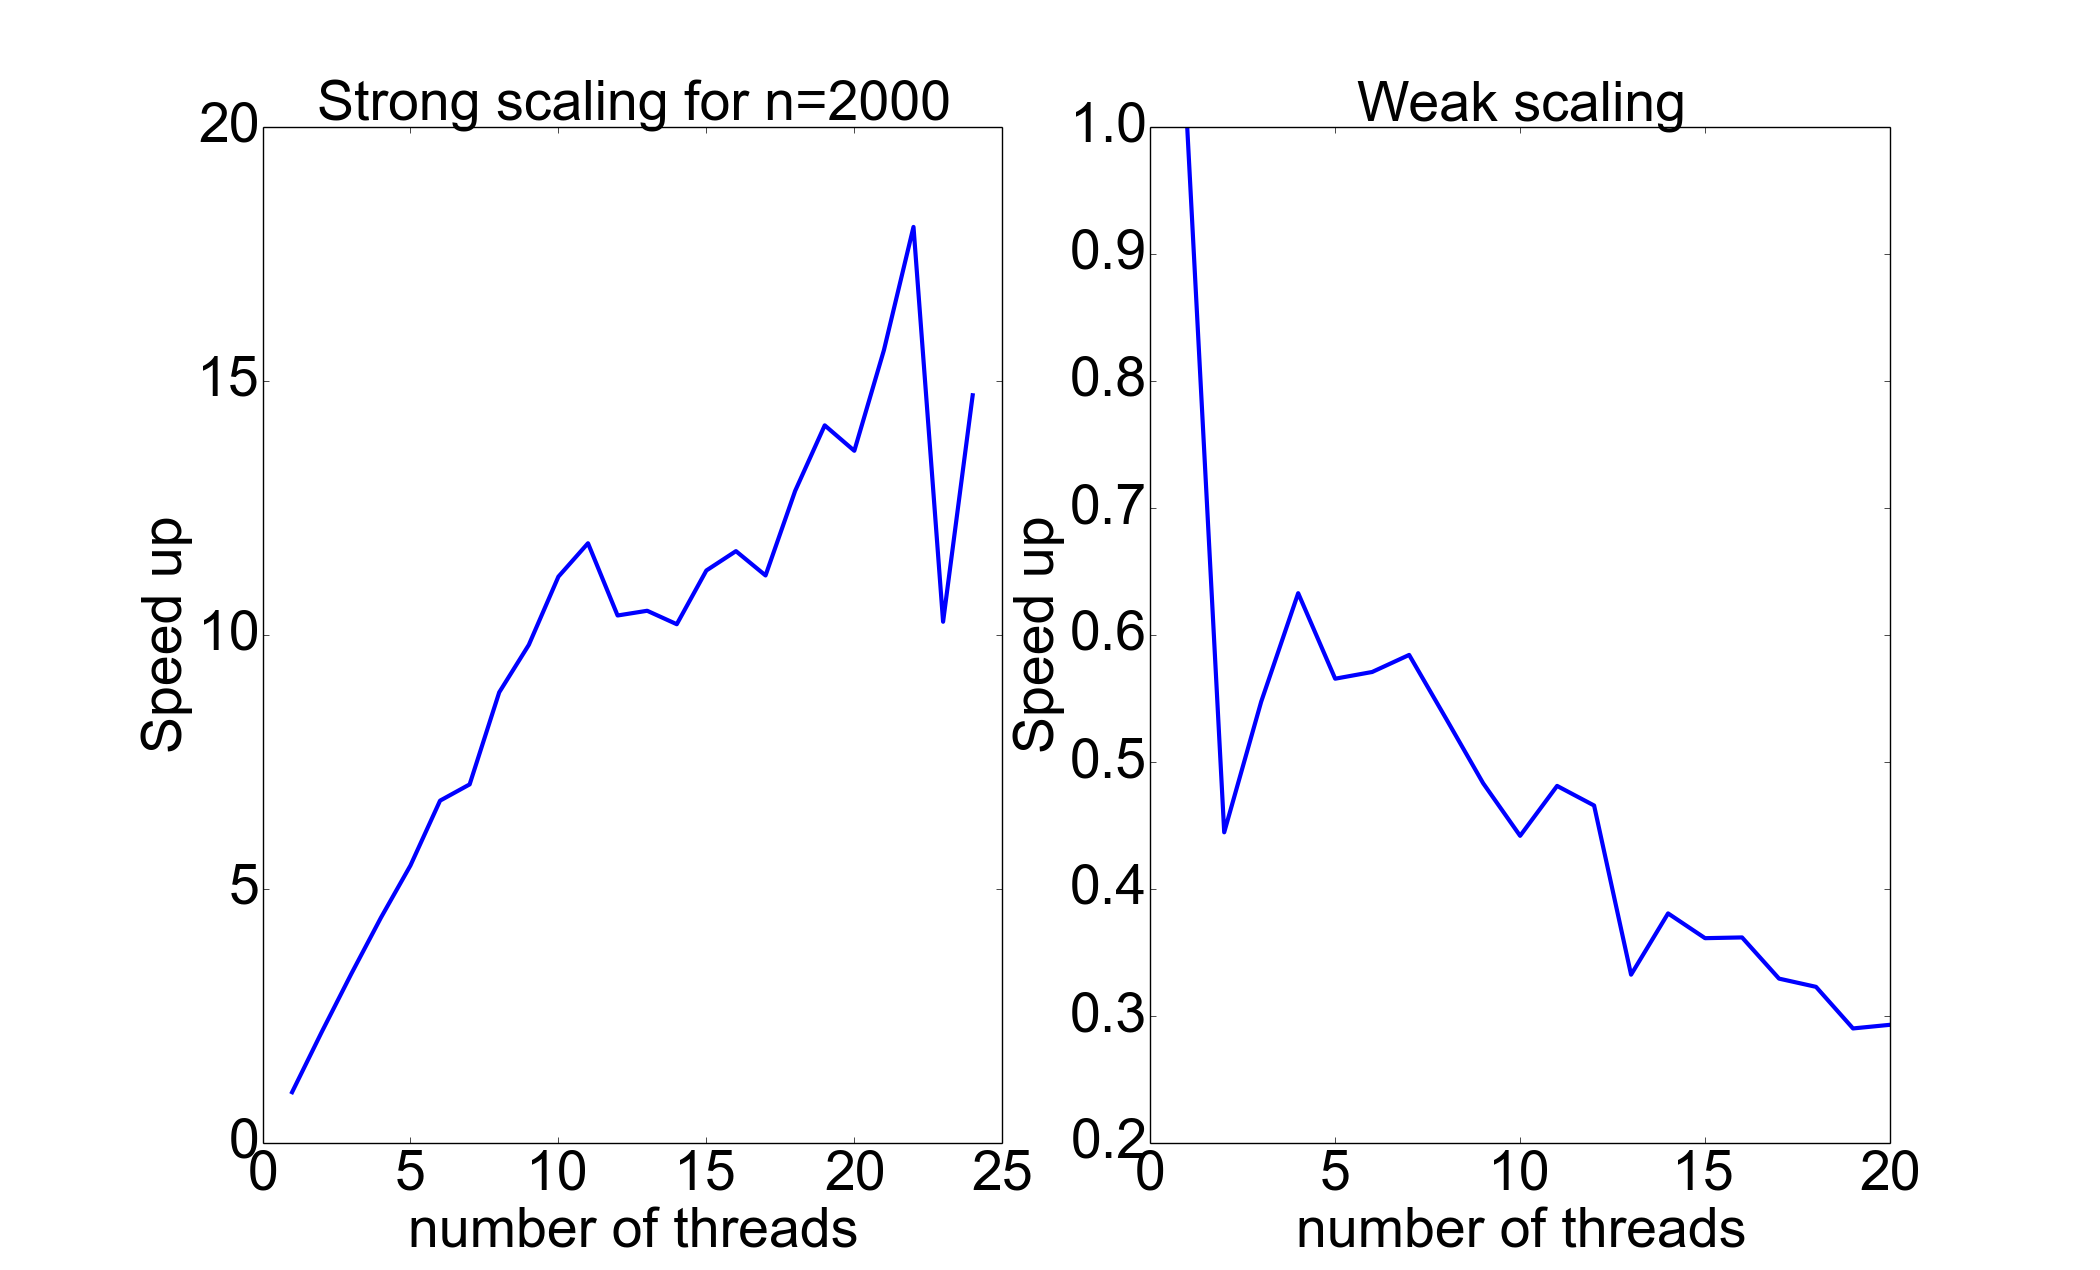
\includegraphics[height=0.4\textwidth, width=\textwidth]{scaling.png}
\end{figure}


\subsection*{Weak Scaling}
In weak scaling, you need to increase both the number of processors and the amount of jobs such that each processor has the same amount of jobs. In this problem, the time complexity is O($n^3 \log n$) and we let each processor has approximately O($2000^3\log(2000)$) amount of work. The results are summarized in the right figure of Figure~\ref{scaling}. As can be seen from the right figure of Figure~\ref{scaling}, the speedup is actually decreasing when you increase the amount of work and the number of processors. This could due to the overheading and synchronization when the number of processors is large.

\section*{MPI Implementation}

We implemented a parallel version of the shortest path algorithm using the
Message Passing Interface (MPI).
In our implementation, each processor is responsible for updating a portion of 
the shortest path matrix $l$.  Specifically, we partition by column, so that 
the processor labelled $k$ (for $k = 1, \ldots, p$), updates $l_{ij}$ for 
$j \in J_k$, where the $(J_k)_{1 \leq k \leq p}$ define a partion of 
$\{1, 2, \ldots, n\}$.
With this strategy the computation pattern for updating the shortest path matrix
remains the same, we are simply looping over a smaller sets of columns.

After each processor has finished updating it's corresponding columns in
the update $l_{ij}^{s+1} = \min_k \{ l^s_{ik} + l^s_{jk} \}$, we call
\emph{MPI\_Allgather} so that each processor gets the fully updated $l^{s+1}$
for the next step.  Each processor also keeps a local ``done'' flag that will
	be true if nothing was updated.  In order to determine whether to terminate
	or not, we call \emph{MPI\_Allreduce} with a logical AND operator on the local
	done flags.


\subsection*{Predicting Speedup}

We considered a simple alpha-beta model to predict the speedup of our MPI implementation.
This models the communication time as
\[ t_{comm} = \alpha + \beta * M \] 
where $\alpha$ is latency, $\beta$ is inverse bandwidth, and $M$ is the message size.
On the totient cluster on a single node, the time per kilobyte to communicate
was previously estimated
\footnote{\url{http://cornell-cs5220-f15.github.io/slides/2015-10-08-model.html}} to be
\[ 0.28 + 0.097 \times kB \quad \mu s \]

Thus the total time for a single iteration
in seconds can be modeled as
\begin{align*}
t_{total} &= t_{serial} + t_{comm} \\
&= O\left(\left(\frac{n}{p}\right)^3\right) 
    + p^2 \frac{0.28 + 0.097(\frac{4n^2}{1000 p})}{10^6}
\end{align*}

We estimated the correct value of $t_{serial}$ by comparing against serial timing 
experiments, and we estimate the number of iterations to be $\log n$.
A plot of estimated speedup for $n=2016$ can be seen in Figure~\ref{mpi-predicted-speedup}.

As seen in the plot, we should expect to get roughly linear speedup up until around 
40 processors, after which communication costs would start to overtake the gains from
paralellization.

Unfortunately, as can be seen in the following section,
the actual results do not match the predicted.  We started seeing the speedup
dropping off when the number of processors was much lower

\begin{figure}
\caption{Predicted MPI Speedup}
\label{mpi-predicted-speedup}
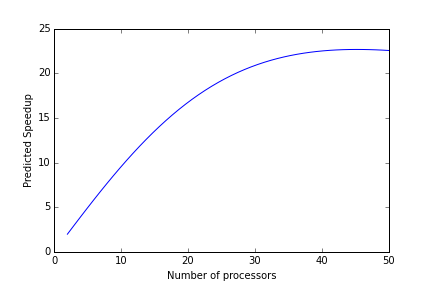
\includegraphics{../results/predicted_speedup.png}
\end{figure}

\subsection*{Scaling Study}

We performed both strong and weak scaling studies for the MPI version of the algorithm.
The results for $n=2016$, averaged over 10 independent trials, can be seen in the Figures
below.  Compared with OpenMP, the MPI version performs relatively poorly in strong scaling 
experiments, but much better in weak scaling experiments for modest number of processors (4-8).

\begin{figure}
\caption{MPI Strong Scaling}
\label{mpi-strong-scaling}
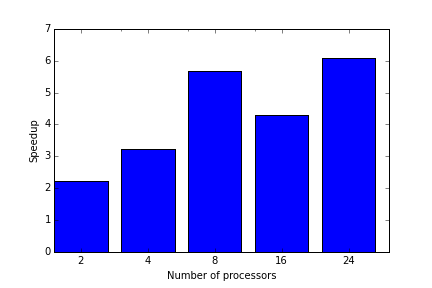
\includegraphics{../results/mpi_strong.png}
\end{figure}

\begin{figure}
\caption{MPI Weak Scaling}
\label{mpi-weak-scaling}
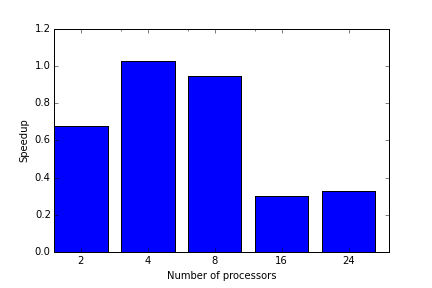
\includegraphics{../results/mpi_weak.png}
\end{figure}

\section*{Tuning}
    We chose to focus on tuning the OpenMP version of the code.\newline

    Since this problem is closely related to the matrix multiplication, we used the same tricks as we did in tuning matrix multiplication, which are copy optimization and blocking. Using copy optimization, we store the transpose of the shortest path matrix to increase the possibility of cache hits. Implementing it will give us 3x to 4x speed up. Similarly, by using blocking, we can better parallellize independent jobs and increase the possibility of cache hits. Combining these two methods together, we achive the speed up seen in Figure~\ref{su}. As you can see, the speedup can be up to 10x. We found the optimal block size to be about 120.\newline

    \begin{figure}
    \caption{speed up for the tuned code}
    \label{su}
    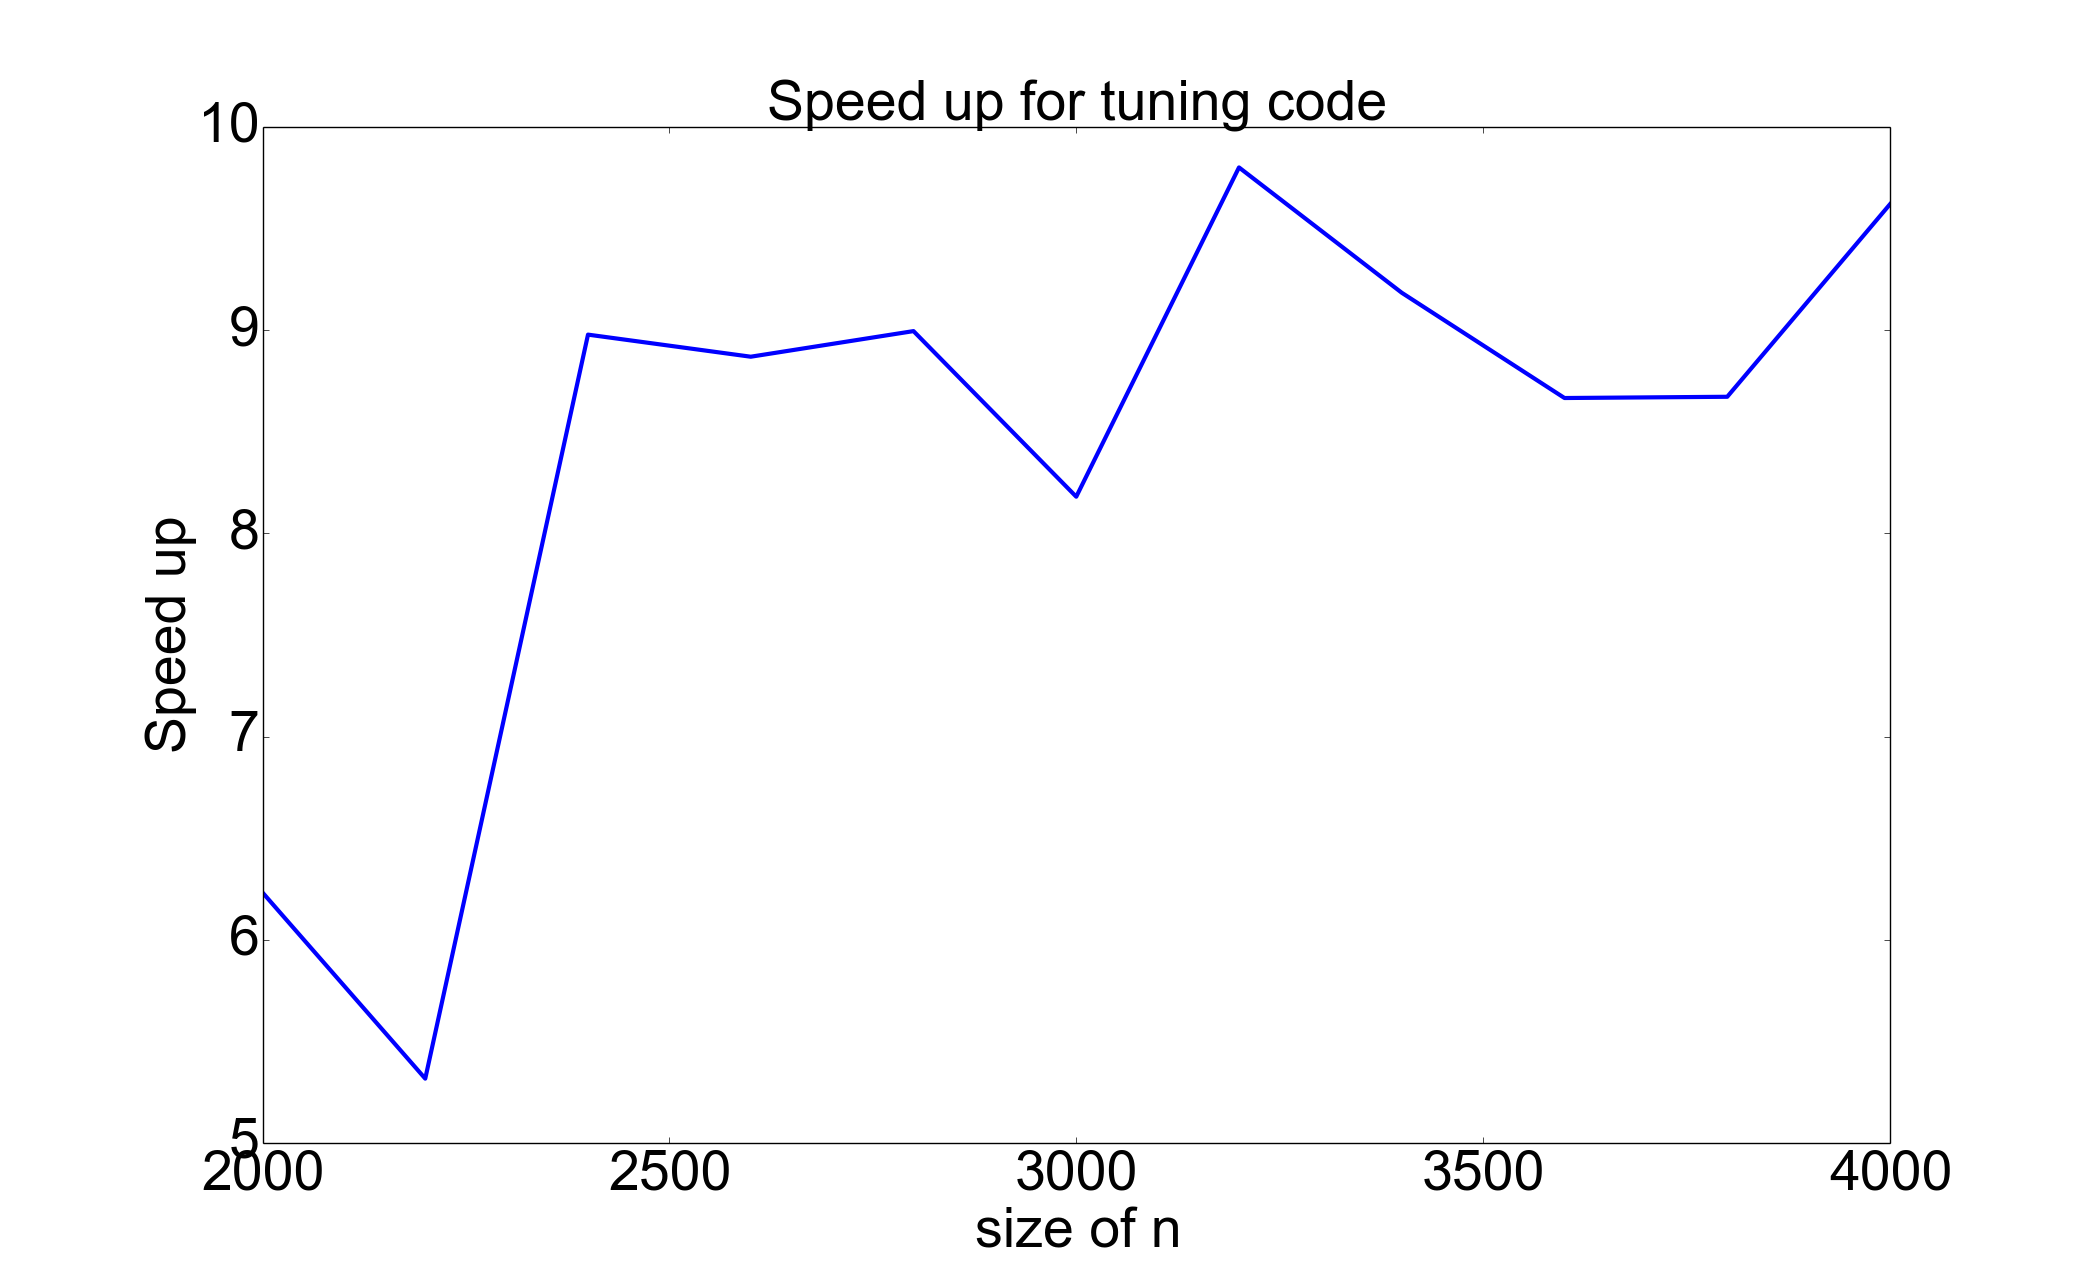
\includegraphics[height=0.4\textwidth, width=\textwidth]{speed_up.png}
    \end{figure}

	The benchmark is the original code using OpenMP with 24 threads.
    
    \begin{figure}[ht!]
    \centering
    \caption{Running VTune Amplifier on optimzed code shows improved memory access}
    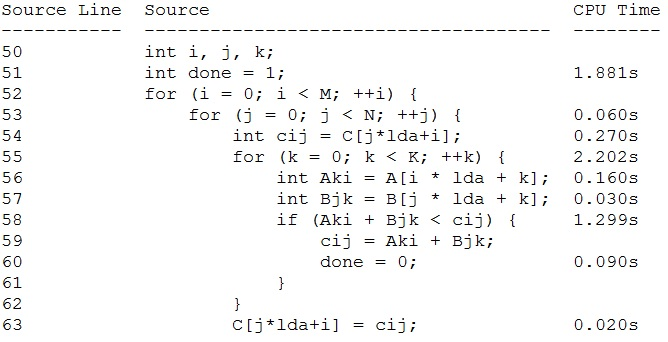
\includegraphics{profileBlocked.jpg}
    \end{figure}
    
    

\end{document}
